% The Artin map factoring through the ray class group:
% I_K(𝔣) ↠ C_K(𝔣) ↠ Gal(L/K), with I_K(𝔣)/H(L/K,𝔣) ≅ Gal(L/K).
% Source: book/tex/alg-NT/artin.tex (§ Artin reciprocity) — tikzcd.
\documentclass[border=2mm]{standalone}
\usepackage{tikz}
\usetikzlibrary{arrows.meta}
\usepackage{amssymb}
\usepackage{amsmath}
\begin{document}
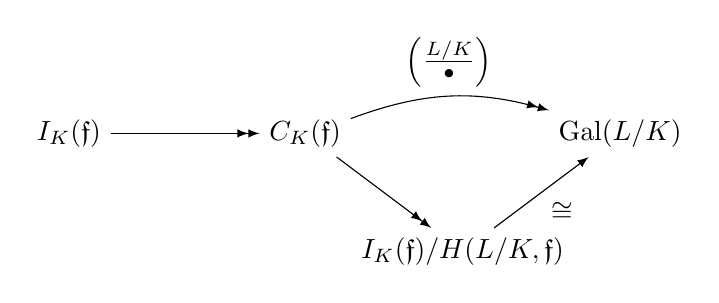
\begin{tikzpicture}[>=latex]
  \node (I) at (0,1.5) {$I_K(\mathfrak{f})$};
  \node (C) at (3,1.5) {$C_K(\mathfrak{f})$};
  \node (G) at (7,1.5) {$\operatorname{Gal}(L/K)$};
  \node (H) at (5,0) {$I_K(\mathfrak{f}) / H(L/K, \mathfrak{f})$};
  \draw[->>] (I) -- (C);
  \draw[->>] (C) to[bend left=18] node[above] {$\left( \frac{L/K}{\bullet} \right)$} (G);
  \draw[->>] (C) -- (H);
  \draw[->] (H) -- (G) node[midway,below right] {$\cong$};
\end{tikzpicture}
\end{document}
